\documentclass[12pt]{article}
%Fall 2022
% Some basic packages
\usepackage{standalone}[subpreambles=true]
\usepackage[utf8]{inputenc}
\usepackage[T1]{fontenc}
\usepackage{textcomp}
\usepackage[english]{babel}
\usepackage{url}
\usepackage{graphicx}
%\usepackage{quiver}
\usepackage{float}
\usepackage{enumitem}
\usepackage{lmodern}
\usepackage{comment}
\usepackage{hyperref}
\usepackage[usenames,svgnames,dvipsnames]{xcolor}
\usepackage[margin=1in]{geometry}
\usepackage{pdfpages}

\pdfminorversion=7

% Don't indent paragraphs, leave some space between them
\usepackage{parskip}

% Hide page number when page is empty
\usepackage{emptypage}
\usepackage{subcaption}
\usepackage{multicol}
\usepackage[b]{esvect}

% Math stuff
\usepackage{amsmath, amsfonts, mathtools, amsthm, amssymb}
\usepackage{bbm}
\usepackage{stmaryrd}
\allowdisplaybreaks

% Fancy script capitals
\usepackage{mathrsfs}
\usepackage{cancel}
% Bold math
\usepackage{bm}
% Some shortcuts
\newcommand{\rr}{\ensuremath{\mathbb{R}}}
\newcommand{\zz}{\ensuremath{\mathbb{Z}}}
\newcommand{\qq}{\ensuremath{\mathbb{Q}}}
\newcommand{\nn}{\ensuremath{\mathbb{N}}}
\newcommand{\ff}{\ensuremath{\mathbb{F}}}
\newcommand{\cc}{\ensuremath{\mathbb{C}}}
\newcommand{\ee}{\ensuremath{\mathbb{E}}}
\newcommand{\hh}{\ensuremath{\mathbb{H}}}
\renewcommand\O{\ensuremath{\emptyset}}
\newcommand{\norm}[1]{{\left\lVert{#1}\right\rVert}}
\newcommand{\dbracket}[1]{{\left\llbracket{#1}\right\rrbracket}}
\newcommand{\ve}[1]{{\bm{#1}}}
\newcommand\allbold[1]{{\boldmath\textbf{#1}}}
\DeclareMathOperator{\lcm}{lcm}
\DeclareMathOperator{\im}{im}
\DeclareMathOperator{\coim}{coim}
\DeclareMathOperator{\dom}{dom}
\DeclareMathOperator{\tr}{tr}
\DeclareMathOperator{\rank}{rank}
\DeclareMathOperator*{\var}{Var}
\DeclareMathOperator*{\ev}{E}
\DeclareMathOperator{\dg}{deg}
\DeclareMathOperator{\aff}{aff}
\DeclareMathOperator{\conv}{conv}
\DeclareMathOperator{\inte}{int}
\DeclareMathOperator*{\argmin}{argmin}
\DeclareMathOperator*{\argmax}{argmax}
\DeclareMathOperator{\graph}{graph}
\DeclareMathOperator{\sgn}{sgn}
\DeclareMathOperator*{\Rep}{Rep}
\DeclareMathOperator{\Proj}{Proj}
\DeclareMathOperator{\mat}{mat}
\DeclareMathOperator{\diag}{diag}
\DeclareMathOperator{\aut}{Aut}
\DeclareMathOperator{\gal}{Gal}
\DeclareMathOperator{\inn}{Inn}
\DeclareMathOperator{\edm}{End}
\DeclareMathOperator{\Hom}{Hom}
\DeclareMathOperator{\ext}{Ext}
\DeclareMathOperator{\tor}{Tor}
\DeclareMathOperator{\Span}{Span}
\DeclareMathOperator{\Stab}{Stab}
\DeclareMathOperator{\cont}{cont}
\DeclareMathOperator{\Ann}{Ann}
\DeclareMathOperator{\Div}{div}
\DeclareMathOperator{\curl}{curl}
\DeclareMathOperator{\nat}{Nat}
\DeclareMathOperator{\gr}{Gr}
\DeclareMathOperator{\vect}{Vect}
\DeclareMathOperator{\id}{id}
\DeclareMathOperator{\Mod}{Mod}
\DeclareMathOperator{\sign}{sign}
\DeclareMathOperator{\Surf}{Surf}
\DeclareMathOperator{\fcone}{fcone}
\DeclareMathOperator{\Rot}{Rot}
\DeclareMathOperator{\grad}{grad}
\DeclareMathOperator{\atan2}{atan2}
\DeclareMathOperator{\Ric}{Ric}
\let\vec\relax
\DeclareMathOperator{\vec}{vec}
\let\Re\relax
\DeclareMathOperator{\Re}{Re}
\let\Im\relax
\DeclareMathOperator{\Im}{Im}
% Put x \to \infty below \lim
\let\svlim\lim\def\lim{\svlim\limits}

%wide hat
\usepackage{scalerel,stackengine}
\stackMath
\newcommand*\wh[1]{%
\savestack{\tmpbox}{\stretchto{%
  \scaleto{%
    \scalerel*[\widthof{\ensuremath{#1}}]{\kern-.6pt\bigwedge\kern-.6pt}%
    {\rule[-\textheight/2]{1ex}{\textheight}}%WIDTH-LIMITED BIG WEDGE
  }{\textheight}% 
}{0.5ex}}%
\stackon[1pt]{#1}{\tmpbox}%
}
\parskip 1ex

%Make implies and impliedby shorter
\let\implies\Rightarrow
\let\impliedby\Leftarrow
\let\iff\Leftrightarrow
\let\epsilon\varepsilon

% Add \contra symbol to denote contradiction
\usepackage{stmaryrd} % for \lightning
\newcommand\contra{\scalebox{1.5}{$\lightning$}}

% \let\phi\varphi

% Command for short corrections
% Usage: 1+1=\correct{3}{2}

\definecolor{correct}{HTML}{009900}
\newcommand\correct[2]{\ensuremath{\:}{\color{red}{#1}}\ensuremath{\to }{\color{correct}{#2}}\ensuremath{\:}}
\newcommand\green[1]{{\color{correct}{#1}}}

% horizontal rule
\newcommand\hr{
    \noindent\rule[0.5ex]{\linewidth}{0.5pt}
}

% hide parts
\newcommand\hide[1]{}

% si unitx
\usepackage{siunitx}
\sisetup{locale = FR}

%allows pmatrix to stretch
\makeatletter
\renewcommand*\env@matrix[1][\arraystretch]{%
  \edef\arraystretch{#1}%
  \hskip -\arraycolsep
  \let\@ifnextchar\new@ifnextchar
  \array{*\c@MaxMatrixCols c}}
\makeatother

\renewcommand{\arraystretch}{0.8}

\renewcommand{\baselinestretch}{1.5}

\usepackage{graphics}
\usepackage{epstopdf}

\RequirePackage{hyperref}
%%
%% Add support for color in order to color the hyperlinks.
%% 
\hypersetup{
  colorlinks = true,
  urlcolor = blue,
  citecolor = blue
}
%%fakesection Links
\hypersetup{
    colorlinks,
    linkcolor={red!50!black},
    citecolor={green!50!black},
    urlcolor={blue!80!black}
}
%customization of cleveref
\RequirePackage[capitalize,nameinlink]{cleveref}[0.19]

% Per SIAM Style Manual, "section" should be lowercase
\crefname{section}{section}{sections}
\crefname{subsection}{subsection}{subsections}
\Crefname{section}{Section}{Sections}
\Crefname{subsection}{Subsection}{Subsections}

% Per SIAM Style Manual, "Figure" should be spelled out in references
\Crefname{figure}{Figure}{Figures}

% Per SIAM Style Manual, don't say equation in front on an equation.
\crefformat{equation}{\textup{#2(#1)#3}}
\crefrangeformat{equation}{\textup{#3(#1)#4--#5(#2)#6}}
\crefmultiformat{equation}{\textup{#2(#1)#3}}{ and \textup{#2(#1)#3}}
{, \textup{#2(#1)#3}}{, and \textup{#2(#1)#3}}
\crefrangemultiformat{equation}{\textup{#3(#1)#4--#5(#2)#6}}%
{ and \textup{#3(#1)#4--#5(#2)#6}}{, \textup{#3(#1)#4--#5(#2)#6}}{, and \textup{#3(#1)#4--#5(#2)#6}}

% But spell it out at the beginning of a sentence.
\Crefformat{equation}{#2Equation~\textup{(#1)}#3}
\Crefrangeformat{equation}{Equations~\textup{#3(#1)#4--#5(#2)#6}}
\Crefmultiformat{equation}{Equations~\textup{#2(#1)#3}}{ and \textup{#2(#1)#3}}
{, \textup{#2(#1)#3}}{, and \textup{#2(#1)#3}}
\Crefrangemultiformat{equation}{Equations~\textup{#3(#1)#4--#5(#2)#6}}%
{ and \textup{#3(#1)#4--#5(#2)#6}}{, \textup{#3(#1)#4--#5(#2)#6}}{, and \textup{#3(#1)#4--#5(#2)#6}}

% Make number non-italic in any environment.
\crefdefaultlabelformat{#2\textup{#1}#3}

% Environments
\makeatother
% For box around Definition, Theorem, \ldots
%%fakesection Theorems
\usepackage{thmtools}
\usepackage[framemethod=TikZ]{mdframed}

\theoremstyle{definition}
\mdfdefinestyle{mdbluebox}{%
	roundcorner = 10pt,
	linewidth=1pt,
	skipabove=12pt,
	innerbottommargin=9pt,
	skipbelow=2pt,
	nobreak=true,
	linecolor=blue,
	backgroundcolor=TealBlue!5,
}
\declaretheoremstyle[
	headfont=\sffamily\bfseries\color{MidnightBlue},
	mdframed={style=mdbluebox},
	headpunct={\\[3pt]},
	postheadspace={0pt}
]{thmbluebox}

\mdfdefinestyle{mdredbox}{%
	linewidth=0.5pt,
	skipabove=12pt,
	frametitleaboveskip=5pt,
	frametitlebelowskip=0pt,
	skipbelow=2pt,
	frametitlefont=\bfseries,
	innertopmargin=4pt,
	innerbottommargin=8pt,
	nobreak=false,
	linecolor=RawSienna,
	backgroundcolor=Salmon!5,
}
\declaretheoremstyle[
	headfont=\bfseries\color{RawSienna},
	mdframed={style=mdredbox},
	headpunct={\\[3pt]},
	postheadspace={0pt},
]{thmredbox}

\declaretheorem[%
style=thmbluebox,name=Theorem,numberwithin=section]{thm}
\declaretheorem[style=thmbluebox,name=Lemma,sibling=thm]{lem}
\declaretheorem[style=thmbluebox,name=Proposition,sibling=thm]{prop}
\declaretheorem[style=thmbluebox,name=Corollary,sibling=thm]{coro}
\declaretheorem[style=thmredbox,name=Example,sibling=thm]{eg}

\mdfdefinestyle{mdgreenbox}{%
	roundcorner = 10pt,
	linewidth=1pt,
	skipabove=12pt,
	innerbottommargin=9pt,
	skipbelow=2pt,
	nobreak=true,
	linecolor=ForestGreen,
	backgroundcolor=ForestGreen!5,
}

\declaretheoremstyle[
	headfont=\bfseries\sffamily\color{ForestGreen!70!black},
	bodyfont=\normalfont,
	spaceabove=2pt,
	spacebelow=1pt,
	mdframed={style=mdgreenbox},
	headpunct={ --- },
]{thmgreenbox}

\declaretheorem[style=thmgreenbox,name=Definition,sibling=thm]{defn}

\mdfdefinestyle{mdgreenboxsq}{%
	linewidth=1pt,
	skipabove=12pt,
	innerbottommargin=9pt,
	skipbelow=2pt,
	nobreak=true,
	linecolor=ForestGreen,
	backgroundcolor=ForestGreen!5,
}
\declaretheoremstyle[
	headfont=\bfseries\sffamily\color{ForestGreen!70!black},
	bodyfont=\normalfont,
	spaceabove=2pt,
	spacebelow=1pt,
	mdframed={style=mdgreenboxsq},
	headpunct={},
]{thmgreenboxsq}
\declaretheoremstyle[
	headfont=\bfseries\sffamily\color{ForestGreen!70!black},
	bodyfont=\normalfont,
	spaceabove=2pt,
	spacebelow=1pt,
	mdframed={style=mdgreenboxsq},
	headpunct={},
]{thmgreenboxsq*}

\mdfdefinestyle{mdblackbox}{%
	skipabove=8pt,
	linewidth=3pt,
	rightline=false,
	leftline=true,
	topline=false,
	bottomline=false,
	linecolor=black,
	backgroundcolor=RedViolet!5!gray!5,
}
\declaretheoremstyle[
	headfont=\bfseries,
	bodyfont=\normalfont\small,
	spaceabove=0pt,
	spacebelow=0pt,
	mdframed={style=mdblackbox}
]{thmblackbox}

\theoremstyle{plain}
\declaretheorem[name=Question,sibling=thm,style=thmblackbox]{ques}
\declaretheorem[name=Remark,sibling=thm,style=thmgreenboxsq]{remark}
\declaretheorem[name=Remark,sibling=thm,style=thmgreenboxsq*]{remark*}
\newtheorem{ass}[thm]{Assumptions}

\theoremstyle{definition}
\newtheorem*{problem}{Problem}
\newtheorem{claim}[thm]{Claim}
\theoremstyle{remark}
\newtheorem*{case}{Case}
\newtheorem*{notation}{Notation}
\newtheorem*{note}{Note}
\newtheorem*{motivation}{Motivation}
\newtheorem*{intuition}{Intuition}
\newtheorem*{conjecture}{Conjecture}

% Make section starts with 1 for report type
%\renewcommand\thesection{\arabic{section}}

% End example and intermezzo environments with a small diamond (just like proof
% environments end with a small square)
\usepackage{etoolbox}
\AtEndEnvironment{vb}{\null\hfill$\diamond$}%
\AtEndEnvironment{intermezzo}{\null\hfill$\diamond$}%
% \AtEndEnvironment{opmerking}{\null\hfill$\diamond$}%

% Fix some spacing
% http://tex.stackexchange.com/questions/22119/how-can-i-change-the-spacing-before-theorems-with-amsthm
\makeatletter
\def\thm@space@setup{%
  \thm@preskip=\parskip \thm@postskip=0pt
}

% Fix some stuff
% %http://tex.stackexchange.com/questions/76273/multiple-pdfs-with-page-group-included-in-a-single-page-warning
\pdfsuppresswarningpagegroup=1


% My name
\author{Jaden Wang}



\begin{document}
\centerline {\textsf{\textbf{\LARGE{Homework 3}}}}
\centerline {Jaden Wang}
\vspace{.15in}

\begin{problem}[1]
\begin{enumerate}[label=(\arabic*)]
	\item Show that $ \widetilde{ \sigma}(s_k)$ is invariant under homotopies of $ s_k$.

		Suppose $ s_k \simeq s_k'$ and $ H: M \times I \to E$ is the homotopy between them. Recall that $ I_i$ is an injection, and let $ j: s_k(M) \to I_i^* E, s_k(m) \to (x, s_k(m))$ where $ I_i(x) = m = p(s_k(m))$ (so $ x$ is unique and $ j$ is well-defined). Clearly $ j$ is also an injection, so the pullback  $ \widetilde{ s_k}$ of $ s_k$ is defined as $ \widetilde{ s_k} = j \circ s_k \circ I_i|_{ \partial e_i^{k+1}}$. Similarly, the pullback $ \widetilde{ s_k'}$ of $ s_k'$ is defined as $ \widetilde{ s_k'} = j \circ s_k' \circ I_i$. Then
		\begin{align*}
			\widetilde{ H}:= j \circ H \circ (I_i, \text{id}_{ [0,1]}): \partial e_i^{k+1} \times [0,1] \to I^* E
		\end{align*}
		is clearly a homotopy between $ \widetilde{ s_k}$ and $ \widetilde{ s_k'}$. Hence $ \widetilde{ s_k} \simeq \widetilde{ s_k'}$. Then clearly $ [p_2 \circ \widetilde{ s_k}] = [p_2 \circ \widetilde{ s_k'}] =: \widetilde{ \sigma}(s_k)$.
	\item $ (\implies):$ suppose $ \widetilde{ g}(s_k) = 0$, then it extends to $ \widetilde{ g}(s_k): e_i^{k+1} \to F$. Since the section is already defined on $ M^{(k)}$, we only need to specify where the $ (k+1)$-cells ( \emph{i.e.} $ I_i(e_i^{k+1})$ for each $ i$) get maps to in  $ E$ via $ s_{k+1}: M^{(k+1)} \to E$. Thus, for each $ I_i(e_i^{k+1})$, let $ \phi: e_i^{k+1} \times F \to I_i^* E$ be the isomorphism. Define
		\begin{align*}
			s_{k+1}|_{I_i(e_i^{k+1})}: I_i(e_i^{k+1}) \to E, x \mapsto \pi_2 \circ \phi \circ ( \text{id}_{ e_i^{k+1}},\overline{ \sigma}(s_k)) \circ  I_i^{-1})(x)
		\end{align*}
		which completes the extension.
	\item $ (\impliedby):$ Suppose $ s_k$ extends over $ M^{(k+1)}$, then we can define $ \widetilde{ s_k}:=j \circ s_k \circ I_i$ without restricting to the boundary, so $  p_2 \circ \widetilde{ s_k}$ can be extended to the entire disk $e_i^{k+1} $. Since $e_i^{k+1} $ is contractible and $ F$ is path-connected (since it is  $ n$-simply connected), the extension of $ p_2 \circ \widetilde{ s_k}$ is null-homotopic and so does $ p_2 \circ \widetilde{ s_k}$. Hence $ \widetilde{ \sigma}(s_k) = 0$.
\end{enumerate}
\end{problem}

\begin{problem}[2]
We wish to show that the join $ S^{m} * S^{n} \cong S^{m+n+1}$.

First recall that $ I^{n} \cong D^{n}$ and $ S^{n} \cong I^{n} / \partial I^{n}$.
~\begin{figure}[H]
	\centering
	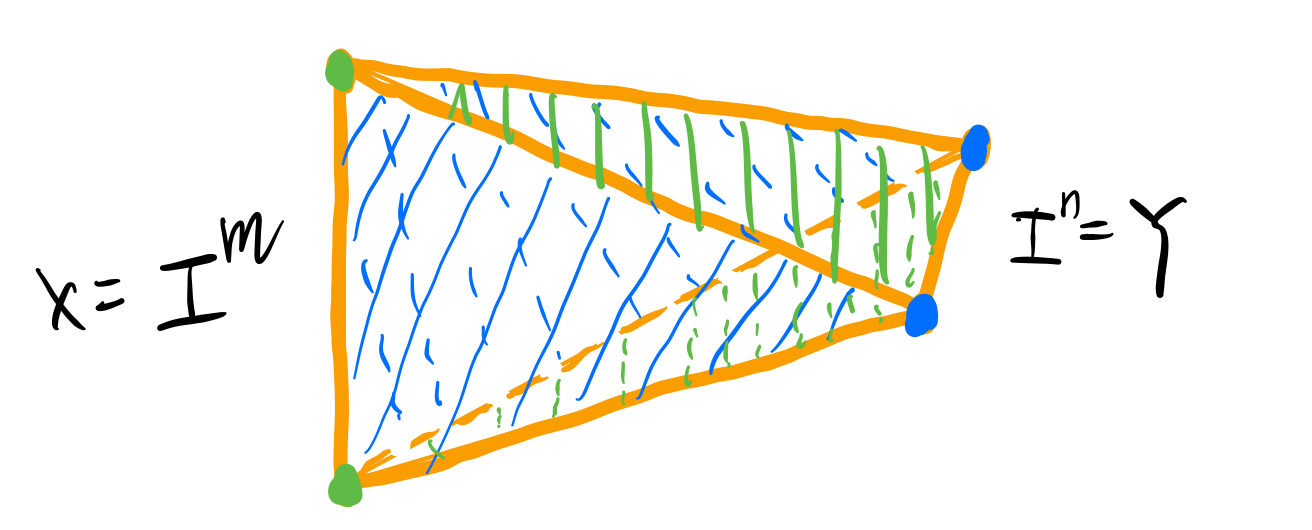
\includegraphics[width=0.8\textwidth]{./figures/join.png}
	\caption{Schematic picture of $ I^{m}*I^{n}$.}
\end{figure}
Note that when $ m=n=1$, the schematic picture of the join is the actual picture. It is easy to see that we obtain a tetrahedron which is homeomorphic to a ball $ D^3$. This easily generalizes to any dimension so we get that $ I^{m} * I^{n} \cong D^{m+n+1}$.

We obtain $ S^{m} * S^{n}$ from $ I^{m} * I^{n}$ by quotienting out the boundaries of both $ I^{m}$ and $ I^{n}$, depicted by green and blue dots. But the whole space traced out by the boundaries in the middle need to be identified as well, depicted by the green and blue shades on the boundaries of the tetrahedron. This forces green and blue to be identified with each other, hence the whole boundary of the tetrahedron is identified. It follows that the quotient map from $ I^{m} * I^{n}$ to $ S^{m} * S^{n}$ is just quotienting the boundary, \emph{i.e.} $ S^{m} * S^{n} \cong I^{m}*I^{n} / \partial (I^{m}*I^{n}) = D^{m+n+1} / \partial D^{m+n+1} \cong S^{m+n+1}$.

In a more rigorous fashion, consider $ S^{m} \subseteq R^{m+1}$, $ S^{n} \subseteq R^{n+1}$, and $ S^{m+n+1} \subseteq \rr^{m+n+2}$. Define
\begin{align*}
	\phi: S^{m}*S^{n}= S^{m} \times I \times S^{n} / \sim \to S^{m+n+1}, [(x,t,y)] \mapsto \cos \left( \frac{t \pi}{ 2} \right) (x,0,0) + \sin \left( \frac{t \pi}{ 2} \right) (0,0,y).
\end{align*}
First we check well-definedness. Since $ (x,0,0),(0,0,y)$ are linearly independent unit vectors, any point in the image can be expressed as
\begin{align*}
	\begin{pmatrix} \cos \frac{t \pi}{ 2} &0\\0& \sin \frac{t \pi}{ 2}  \end{pmatrix} \begin{pmatrix} x\\y \end{pmatrix} =: D(t) \begin{pmatrix} x\\y \end{pmatrix} 
\end{align*}
Since $ D(t)$ is clearly a unitary matrix, the image lies on the unit sphere of $ \rr^{m+n+2}$. Given representatives $ (x,0,y_1)$ and $ (x,0,y_2)$, we see that $ \sin \left( \frac{0 \cdot  \pi}{2 } \right) =0$ so they give the same output. Similarly, $ (x_1,0,y)$ and $ (x_2,0,y)$ give the same output. Hence $ \phi$ is well-defined.

Next, we show that $ \phi$ is injective. Suppose
\begin{align*}
	\cos \left( \frac{t_1 \pi}{ 2} \right) x_1 + \sin \left( \frac{t_1 \pi}{ 2} \right) y_1 &= \cos \left( \frac{t_2 \pi}{ 2} \right) x_2 + \sin \left( \frac{t_2 \pi}{ 2} \right) y_2 
\end{align*}
When $ t_1 , t_2 \neq 0,1$, since $ \cos \left( \frac{t_1 \pi}{ 2} \right) x_1 - \cos \left( \frac{t_2 \pi}{ 2} \right) x_2$ and $ \sin \left( \frac{t_1 \pi }{ 2}  \right)y_1 - \sin \left( \frac{t_2 \pi}{ 2} \right) y_2 $ are linearly independent, this forces each term to be 0. Moreover, $ x_1 \neq x_2$ and $ y_1 \neq y_2$ are on spheres and thus linearly independent unless they are antipodal, but the coefficients stay within $ [0,1]$ so they cannot be antipodal. That is, the only way for each term to be 0 is when $ x_1 = x_2$ and $ y_1 = y_2$. Since they are on spheres, the coefficients must equal as well, and on $ [0, \pi /2)$ the  $ \cos$ function is invertible and so is $ \sin$ on $ (0, \pi /2]$, so $ t_1 = t_2$.

When $ t_1 = 0$ or 1, it forces $  t_2 = t_1$ by linear independence. We see that $ y_1,y_2$ can be anything when $ t=0$ and  $ x_1 ,x_2$ can be anything when $ t=1$, but they are in the same equivalence class here so injectivity still holds.

Then we show that  $ \phi$ is surjective. Given a point $ p \in S^{m+n+1}$, we simply project $ p$ to $ \rr^{m}$ and $ \rr^{n}$ identified as subspaces of $ \rr^{m+n+1}$ and scale the images so they have unit length and lie in the same quadrant, called $ x$ and  $ y$. Then $ p$ is on the ``circular" path of these two points and therefore has a point $ (x,t,y)$ mapping to  $ p$ via $ \phi$. 

Since the continuity of $ \phi$ is immediate from the continuity of trig functions and quotient map, $ \phi$ is bijective continuous. As $ \rr^{m+n+2}$ is Hausdorff and $ S^{m}*S^{n}$ is compact, we conclude that $ \phi$ is a homeomorphism.
\end{problem}
\begin{problem}[3]
If $ 0 \to B \to A \xrightarrow{ j}  C \to 0$ is exact and $ C$ is free, then  $ A \cong B \oplus C$.

By exactness, $ j$ is surjective so for every $ c \in C$, $ j^{-1}(c) \neq \O$. Since $ C$ is free, it has a basis $ S$ and we can define a module homomorphism $ t: C \to A$ by the set map $ S \to A, s \mapsto \widetilde{ s}$ where $ \widetilde{ s} \in j^{-1}(s)$ by the universal property of free modules. It follows that
\begin{align*}
	j \circ t (s) = j(\widetilde{s }) = s = \text{id}_{ C}(s).
\end{align*}
Hence the sequence splits and the claim follows. More specifically, the short exact sequence implies that $ C \cong A / B$ where $ B$ is identified as  $ \im i$. By $ t$, we can identify  $ C$ as a submodule of  $ A$. It is easy to see that  $ B \cap C = \{0\}$ and $ B+C = A$ by taking a representative in  $ C$ and an element of  $ B$. Hence  $ A = B \oplus C$.
\end{problem}

\begin{problem}[4]
Here we prove part 3 and 4 of Lemma IV.1.

Suppose $ F$ is a finite filtration of  $ A$.

3): if $ G(A)_s$ is finite for all  $ s$, then we know that $ G(A)_0 =  F_0A / F_{-1}A = F_0A / 0 \cong F_0 A$ is finite with order $ n_0$. Since $ G(A)_1 = F_1A / F_0A $ is also finite with order $ n_1$, viewing the modules as abelian groups we have $ |F_1A| = |F_0A| |F_1 A / F_0 A| = n_0 n_1$ by Lagrange. If $ t$ is the index such that $ F_t A = A$, then inductively it is easy to see that $ |A| = |F_t A | = |F_{t-1} A| |G(A)_t| = \prod_{ s= 0}^{ t} n_s$ which is finite. Moreover, $ G(A) = \bigoplus_{ s=0}^{t} G(A)_s \cong \prod_{ s= 0}^{ t} G(A)_s$ by finiteness of $ G(A)_s$ so  $ |G(A)| = \prod_{ s= 0}^{ t} |G(A)_s| = \prod_{ s= 0}^{ t} n_s = |A|$.

4): if $ G(A)_s$ is finitely generated for all  $ s$, by a theorem from algebra, we know that if modules $ N$ and  $ M /N$ are finitely generated, so is  $ M$, which is generated by generators of $ N$ and representatives of generators of  $ M /N$. Since the rank of a module is the cardinality of maximal free generating set of the module, free generators of $ N$ and  $ M /N$ are still generators of  $ M$ but might not be free, so $ \rank M \leq \rank N + \rank M /N$. But we see that they are indeed free in $ M$, since if $ B = \{b_1,\ldots,b_n\} $ is the maximal free generators of  $ N$ and  $ A = \{\overline{a_1},\ldots,\overline{a_m}\} $ is that of $ M /N$, then we see that if
\begin{align*}
	c_1 a_1 + \cdots c_m a_m + d_1 b_1 + \cdots + d_n b_n &= 0 \\
	c_1 a_1 + \cdots c_m a_m &= -d_1 b_1 - \cdots d_n b_n \in N
\end{align*}
This forces $ c_1 = \ldots=c_m = 0$ by $ A$ being a linearly independent set of  $ M /N$. It follows that  $ d_1 = \cdots = d_n = 0$ by $ B$ being a linearly independent set of  $ N$. So we conclude that the set $ \{a_1,\ldots,a_m,b_1,\ldots,b_n\} $ is a linearly independent set of $ M$, so  $ \rank M \geq \rank N + \rank M /N$ which yields equality. By induction we easily see that  $ \rank (A) = \sum_{ s= 0}^{ t} \rank (G(A)_s)$. Since the filtration is finite, direct sum is isomorphic to direct product, so we quickly see that free generators of each component remains free in the direct product and hence in the direct sum. That is, $ \rank (G(A)) = \bigoplus_{ s=0}^{t} \rank (G(A)_s) = \rank A$.
\begin{align*}
	c_1 a_1 
\end{align*}
\end{problem}
\end{document}
